% Technische Universität Dresden
% Fakultät Informatik
% Institut für Software- und Multimediatechnik
% Seniorprofessur für Multimediatechnik
%
% Example document demonstrating the usage of mmthesis.sty
% 2012-10-26 Andreas Rümpel
% 
% ### build hints (% = filename of tex file) ###
% pdflatex: pdflatex %.tex
% biber: biber % (biber is a modern backend for bibtex, http://biblatex-biber.sourceforge.net)
% glossaries and acronyms: makeglossaries %
%
% Das LATEX2e-Sündenregister: ftp://ftp.dante.de/tex-archive/info/l2tabu/german/l2tabu.pdf
% KOMAScript-Guide: ftp://ftp.dante.de/tex-archive/macros/latex/contrib/koma-script/scrguide.påådf
% Einige typographische Grundregeln und ihre Umsetzung in LaTeX: http://www2.informatik.hu-berlin.de/sv/lehre/typographie.pdf

\documentclass[
	headsepline,
	footsepline,
	fontsize=12pt,
	%draft, % use this for finding overfull boxes
	%parskip, % use this for alternative paragraph formatting
	bibliography=totoc
]{scrbook}

\usepackage{mmthesis}
\addbibresource{library.bib} % put name of bib file here with extension

%### switches
%\printoutput % make link colors black, leave deactivated for screen output

%### define metadata
\mmtype{Diplomarbeit} %Diplomarbeit|Großer Beleg|Bachelorarbeit|Masterarbeit|Seminararbeit
\mmtitle{Semantik-gestütztes Hilfesystem für ein komposites Informationsvisualisierungssystem}
\mmtshorttitle{Hilfesystem für komposite InfoVis}
\mmtauthor{Nikolaus Piccolotto}
\mmtsubmissionmonth{November 2013}
\mmtsubmissiondate{30. November 2013}
\mmtsupervisor{Dipl.-Medieninf. Martin Voigt}
%\mmtsupervisorii{Dipl.-Medieninf. Foo Bar} % Co-supervisor, optional

\mmthypersetup % has to be called after setting metadata

%### acronyms
\newacronym{PDF}{PDF}{Portable Document Format}
\newacronym{RCP}{RCP}{Rich Client Platform}
\newacronym{RIA}{RIA}{Rich Internet Application}
\newacronym{RELAXNG}{RELAX NG}{Regular Language Description for XML New Generation}
\newacronym{SGML}{SGML}{Standard Generalized Markup Language}
\newacronym{SWT}{SWT}{Standard Widget Toolkit}
\newacronym{WDC}{W3C}{World Wide Web Consortium}
\newacronym{WPF}{WPF}{Windows Presentation Foundation}
\newacronym{XPath}{XPath}{XML Path Language}
\newacronym{XHTML}{XHTML}{Extensible Hypertext Markup Language}
\newacronym{XML}{XML}{Extensible Markup Language}
% my acronyms
\newacronym{InfoVis}{InfoVis}{Informationsvisualisierung}

\begin{document}
\frontmatter
\pagenumbering{Roman}
\mmtfrontmatter

\listoffigures
\listoftables
\printglossary[type=\acronymtype,style=long,title=Abkürzungsverzeichnis,toctitle=Abkürzungsverzeichnis]
%\printglossary %Glossar

\mainmatter

% ###################################################
\chapter{Einleitung}
\label{chapter:einleitung}

% Hier kommt eine kurze Einführung von semantischen Daten, nehme ich an

% ###################################################
\section{Motivation}
\label{section:motivation}

% Hier wird generell eingeleitet, also vermutlich die Problematik zwischen semantischen Datensätzen und Endusern

% ###################################################
\section{Problemstellung und Zielsetzung}
\label{section:problemstellung}

% Hier wird quasi der Vizboard Workflow umrissen
% und erklärt, wo das eigentliche Problem liegt, nämlich im Information Overload beim letzten Schritt

\begin{figure}[htbp]
	\centering
	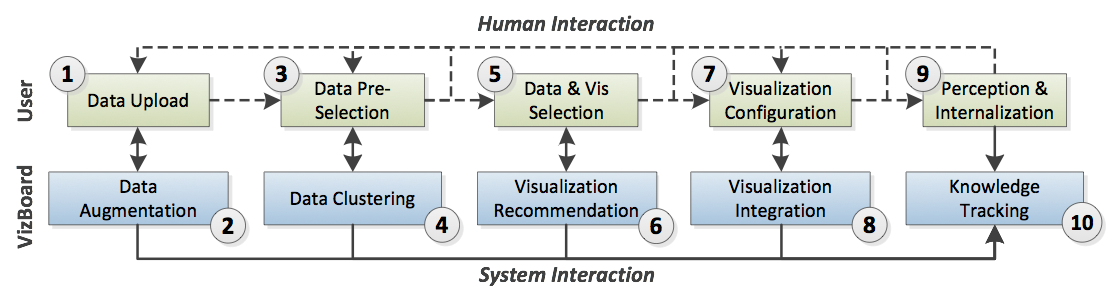
\includegraphics[width=0.75\textwidth]{images/vizboard_workflow.png}
	\caption{VizBoard Workflow}
	\label{figure:vizboard_workflow}
\end{figure}

% ###################################################
\section{Aufbau der Arbeit}
\label{section:aufbau}

% Aufbau der Arbeit erklären, kommt zum Schluss

% ###################################################
\chapter{Stand der Forschung und Technik}
\label{chapter:standderforschung}

Der folgende Abschnitt besteht aus drei Teilen. Zuerst wird die Aufgabenstellung in einem Szenario verdeutlicht (Abschnitt~\ref{section:szenario}). Daraus werden Anforderungen an das Hilfesystem abgeleitet (Abschnitt~\ref{section:anforderungsanalyse}) und danach die Grundlagen von semantischen Daten, Informationsvisualisierungen und Software Support erläutert (Abschnitt~\ref{section:grundlagen}).

% ###################################################
\section{Szenario}
\label{section:szenario}

% kurze einleitung noch mal

Wie in Kapitel~\ref{chapter:einleitung} erläutert, ist das komposite InfoVis-System Teil der webbasierten Anwendung VizBoard. Sie leitet den Benutzer in mehreren Schritten von der Auswahl eines Datensatzes zur finalen, kompositen Informationsvisualisierung. Im vorletzten Schritt wählt dieser mit Hilfe eines Facettenbrowsers geeignete Visualisierungskomponenten aus, welche danach angezeigt werden. Um die Problemstellung noch einmal zu verdeutlichen, wird im folgenden ein mögliches Szenario beschrieben.

% einführung der problemstellung
Anna möchte für ihr Biologiestudium mehr über die geografische Verteilung verschiedener Genvarationen herausfinden. Dazu sucht sie im Internet nach einem Datensatz, welchen sie auch findet. 
% unbekanntes format, kann es nirgends ordentlich öffen und selbst wenn es in excel ginge, wüsste sie nicht, welche charts sie am besten erstellen sollte
Leider ist er in einem für Anna unbekannten Format abgespeichert, nämlich OWL. Sie versucht die Datei mit Microsoft Excel und SPSS zu öffnen, weil sie keine anderen Programme zur Datenverarbeitung kennt, aber scheitert. Anna stellt fest, dass nur ihr Texteditor OWL öffnen und vernünftig darstellen kann. Als sie die Datei überfliegt, kann sie den Inhalt zwar erahnen, aber es ist einfach zu viel Text um ihn vollständig zu lesen. Davon abgesehen sind geografische Breite und Länge als Zahlenkombination keine anschauliche Repräsentation von Orten, auch Verteilungen von Werten sind so schwer ersichtlich. Anna würde viel Zeit aufwenden müssen um sehr wenig des Inhalts zu verstehen. Aber selbst wenn sie die Datei in Excel hätte öffnen können, hätte sie nicht gewusst, mit welchen Diagrammen die vorhandenen Daten am Besten verstanden würden. Anna hört von einem Freund, dass VizBoard gut geeignet ist, um semantische Datensätze anzusehen und probiert es aus.

% Der Benutzer ist laut unserem Rollenmodell weder Developer noch Visualisierungsexperte, d.h. er hat erstmal Schwierigkeiten zu erfassen, was hier überhaupt abgeht

Anna hat ihren Datensatz auch bei VizBoard gefunden und ist neugierig: Sie wählt eine Karte, ein Balkendiagramm, eine Tabelle und eine Treemap aus (Abbildung~\ref{figure:szenario-skizze}); kurz darauf werden ihr die Visualisierungskomponenten angezeigt. Anna benutzt VizBoard zum ersten Mal und macht außer Facebook und YouTube auch sonst nicht viel im Internet, das heißt sie ist zunächst von den vier unterschiedlichen Fenstern etwas überfordert.

\begin{figure}[htbp]
	\centering
	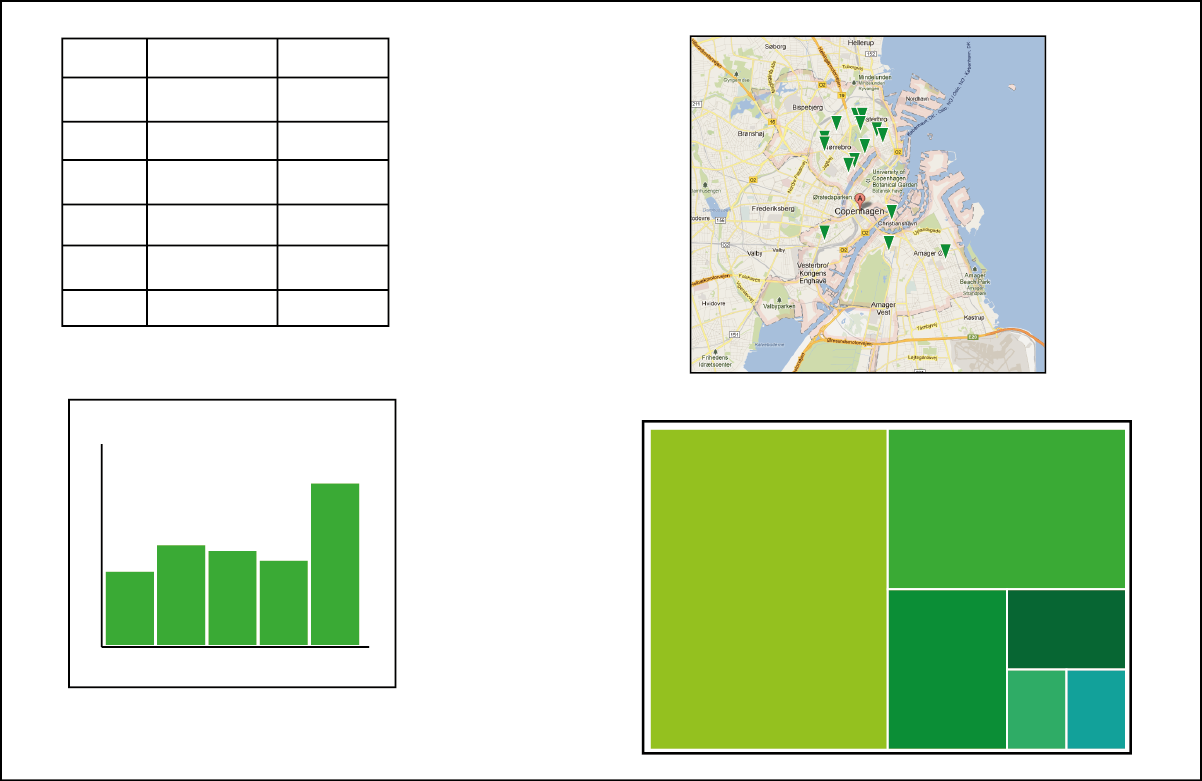
\includegraphics[width=0.75\textwidth]{images/szenario-skizze.png}
	\caption{Skizze der VizBoard Visualisierungskomponenten}
	\label{figure:szenario-skizze}
\end{figure}

VizBoard bietet Anna aber sofort eine einführende Übersicht und erklärt kurz die Darstellungsform und den Inhalt jeder Komponente. Eine denkbare Erklärung der Treemap wäre zum Beispiel:

\begin{quote}
Eine Treemap ist eine hierarchische Visualisierung, um Größenverhältnisse anschaulich zu machen. In dieser werden die Anzahl von Genvariationen pro geografischer Region dargestellt.
\end{quote}

% Was sind das für Fenster? Welche Komponente ist welche? Welche macht was? Wie kann ich sie bedienen? HUUUPS da ändert sich ja was obwohl ich dort nix gemacht hab! Wie hängen die zusammen? Was sind das für Daten, die dargestellt werden? 

Damit bekommt Anna einen Überblick über die verfügbaren Visualisierungen und weiß, welches Fenster welche Visualisierung enthält und für was diese gut sind. Nun möchte sie die Tabelle, in der die durch die Treemap visualisierten Daten stehen, nach der Spalte \enquote{Anzahl} sortieren. Anna sieht aber nicht, wie sie das machen soll, da in der Tabelle kein offensichtliches Kontrollelement wie z.\,B. ein Button vorhanden ist. Sie bemerkt ein Fragezeichen in der Titelleiste des Fensters und klickt darauf. Der verfügbare Viewport wird abgedunkelt und es erscheint ein neues Fenster, welches die verfügbaren Aktionen mit Hilfe von Text, Bildern und Animationen erklärt. Anna lernt, dass sie mit einem einfachen Linksklick auf den jeweiligen Kopf einer Tabellenspalte nach dieser sortieren kann und außerdem eine oder mehrere Zeilen auswählen kann. Sie sortiert die Tabelle wie gewollt und wählt die ersten drei Zeilen aus. Plötzlich verkleinert die Karte ihr Zoomlevel und Anna ist verwirrt: Sie hat nur mit der Tabelle interagiert und es bestand keine sichtbare Verbindung zwischen den beiden Fenstern. Allerdings wurde nach der Zeilenauswahl ein Pfeil von der Tabelle zur Karte gezeichnet, welcher mit einem Icon in Form eines Briefes versehen ist. Anna vermutet, dass doch irgendeine Verbindung zwischen den beiden Visualisierungen besteht und klickt auf den Brief. Ähnlich wie vorhin bei der Hilfe zur Tabelle wird der Viewport abgedunkelt und ein neues Fenster wird eingeblendet. Es erklärt die Kommunikation zwischen den Visualisierungen mit Hilfe von Animationen, Text und Bildern. Nun weiß Anna auch, wie die verschiedenen Fenster zusammenhängen und kann sich ihrer eigentlichen Aufgabe widmen.

% Was heißt GDP? Wie wird das berechnet? Was soll die Spitze bei 1990? Woher kommt die? Diese eine Komponente scheint kaputt zu sein, wo kann ich mich beschweren?

In der Tabelle findet sie auch eine Spalte \enquote{SNP}. Anna weiß zwar, dass sie die Abkürzung schon einmal gesehen hat, kennt aber im Moment ihre Bedeutung nicht. Praktischerweise ist der Spaltenkopf mit der Wikipedia verlinkt und sie wird sofort auf die entsprechende Seite weitergeleitet. Anna erinnert sich, dass \enquote{SNP} \enquote{Single-nucleotide polymorphism} bedeutet und sie bekommt auch gleich zusätzliche Informationen zu diesem Thema. Sie widmet sich weiter der Tabelle und stellt fest, dass die Ortsbezeichnung \enquote{Kopenhagen} nicht mit der Markierung in der Karte übereinstimmt. Außerdem ist sie erstaunt, wie hoch die Verbreitung eines bestimmten SNPs dort ist und würde gerne die Ursache dafür wissen. In der Hilfe zur Tabelle wurde sie auch über die Möglichkeit, Kommentare an den Daten vorzunehmen, aufgeklärt. Anna kommentiert sowohl die falschen Geokoordinaten als auch ihre Frage über die Verbreitung des SNPs, sodass sie später über Antworten informiert wird. Nun kann Anna sich mit der vierten Visualisierung, dem Balkendiagramm, beschäftigen. Allerdings reagiert es auf keine Mausklicks und macht auch sonst nicht den Eindruck, die Daten akkurat darzustellen. Anna meldet die kaputte Visualisierung über die eingebaute Reporting-Funktion und schließt das Fenster, um sich den anderen drei Visualisierungskomponenten zuzuwenden.

% ###################################################
\section{Anforderungsanalyse}
\label{section:anforderungsanalyse}

Aus dem Szenario (Kapitel~\ref{section:szenario}) lassen sich nun verschiedene Anforderungen an ein Hilfesystem für komposite Informationsvisualisierungssysteme ableiten.

\subsection{Funktionale Anforderungen}
\label{section:funktionale_anforderungen}

Blabla

\begin{itemize}
	\item\textbf{Überblick}: Das Hilfesystem soll einen kurzen Überblick über das InfoVis-System geben und Darstellungsform sowie Inhalt jeder Komponente kurz erläutern.
	\item\textbf{Bedienung}: Das Hilfesystem soll erklären können, wie eine Komponente bedient wird. Diese Informationen umfassen beispielsweise welche Operationen welche Aktionen (eventuell auf welchen Daten) ausführen.
	\item\textbf{Reporting}: Fehler in Komponenten sollen über ein Reporting-System gemeldet werden können.
	\item\textbf{Verlinkung}: Das Hilfesystem soll nicht-triviale Begriffe mit einer Wissensbasis‚ verlinken, sodass nicht nur auf die Begriffsbedeutung hingewiesen werden, sondern dem Benutzer auch zusätzliche Informationen zur Verfügung gestellt werden können.
	\item\textbf{Kommunikation}: Das Hilfesystem soll erklären können, wie gegebene Komponenten miteinander kommunizieren.
	\item\textbf{Kommentare}: Der Benutzer soll die Möglichkeit haben Daten zu kommentieren und Bereiche der Visualisierung zu markieren und mit ebenfalls mit einem Kommentar zu versehen, sodass auch auf fehlende Daten hingewiesen werden kann.
\end{itemize}

% was muss also ins related work?
% wie der wissensaufnahmeprozess funktioniert, weil ich ja erklärungen gebe, speziell planerklärung
% was es so für infovis gibt, weil ich mit denen arbeite
% was es so für hilfekonzepte gibt, weil es das ist was ich tue
% social web, weil kommentare implementiert werden

\subsection{Nichtfunktionale Anforderungen}
\label{section:nichtfunktionale_anforderungen}

Bla bla

\begin{itemize}
	\item\textbf{Korrektheit}: Eine gegebene Hilfestellung darf keine Fehlinformationen enthalten, weil sie sonst mehr verwirrt als hilft.
	\item\textbf{Vollständigkeit}: Eine gegebene Hilfestellung muss alle Informationen enthalten, die der Nutzer benötigt um danach seine gewünschte Aufgabe ausführen zu können.
	\item\textbf{Verständlichkeit}: Hilfestellungen müssen in einer Form präsentiert werden, die der Benutzer schnell und mit geringem mentalen Aufwand verarbeiten kann.
	\item\textbf{Einheitlichkeit}: Das Look \& Feel von Teilen des Hilfesystems (z.B. Kommentare) muss komponentenübergreifend einheitlich sein, damit der Benutzer einmal gelerntes wiederverwenden kann.
	\item\textbf{Minimalität}: Der Komponentenentwickler soll seine Komponente mit möglichst wenig Aufwand zum Hilfesystem kompatibel machen können, ansonsten werden nur sehr wenige Komponenten -- und damit der Benutzer -- davon profitieren.
	\item\textbf{Universalität}: Das Hilfesystem soll für alle Komponenten und Visualisierungen in gleicher Qualität funktionieren.
	\item\textbf{Wiederverwendbarkeit}: Die Kommentare sollen möglichst in allen Visualisierungen wiederverwendet werden, damit viele Benutzer von den Erkenntnissen anderer profitieren können.
	\item\textbf{Unaufdringlichkeit}: Das Hilfesystem soll den Benutzer nicht von seinen Aufgaben ablenken und nur auf Anfrage zum Einsatz kommen oder es soll selbständig erkennen, wenn der Benutzer Hilfe benötigt.
\end{itemize}

% ###################################################
\section{Grundlagen}
\label{section:grundlagen}

Hurrrrr derp herp

\subsection{CRUISe, EDYRA \& VizBoard}
\label{section:vizboard}

% grundlagen von cruise edyra vizboard. wichtig weil mein hilfesystem dort eingesetzt wird
CRUISe \cite{Pietschmann2009, Pietschmann2012} ist ein Framework zur Konstruktion von sogenannten Mashup User Interfaces. Diese bestehen aus mehreren voneinander unabhängigen, wiederverwendbaren User Interface Services (z.\,B. eine Karte, eine Tabelle und ein Kalender) welche zur Laufzeit hinzugefügt, konfiguriert und ausgetauscht werden können. Abbildung~\ref{figure:cruise_architektur} zeigt die Architektur von CRUISe. Zuerst werden Komponenten von Entwicklern erstellt und modelliert (1). Danach interpretiert CRUIse das Kompositionsmodell (2), matcht es gegen die Kontextanforderungen (3), bildet ein Ranking (4) und integriert schließlich die am besten geeignete Komponente ins User Interface (5).

\begin{figure}[htbp]
	\centering
	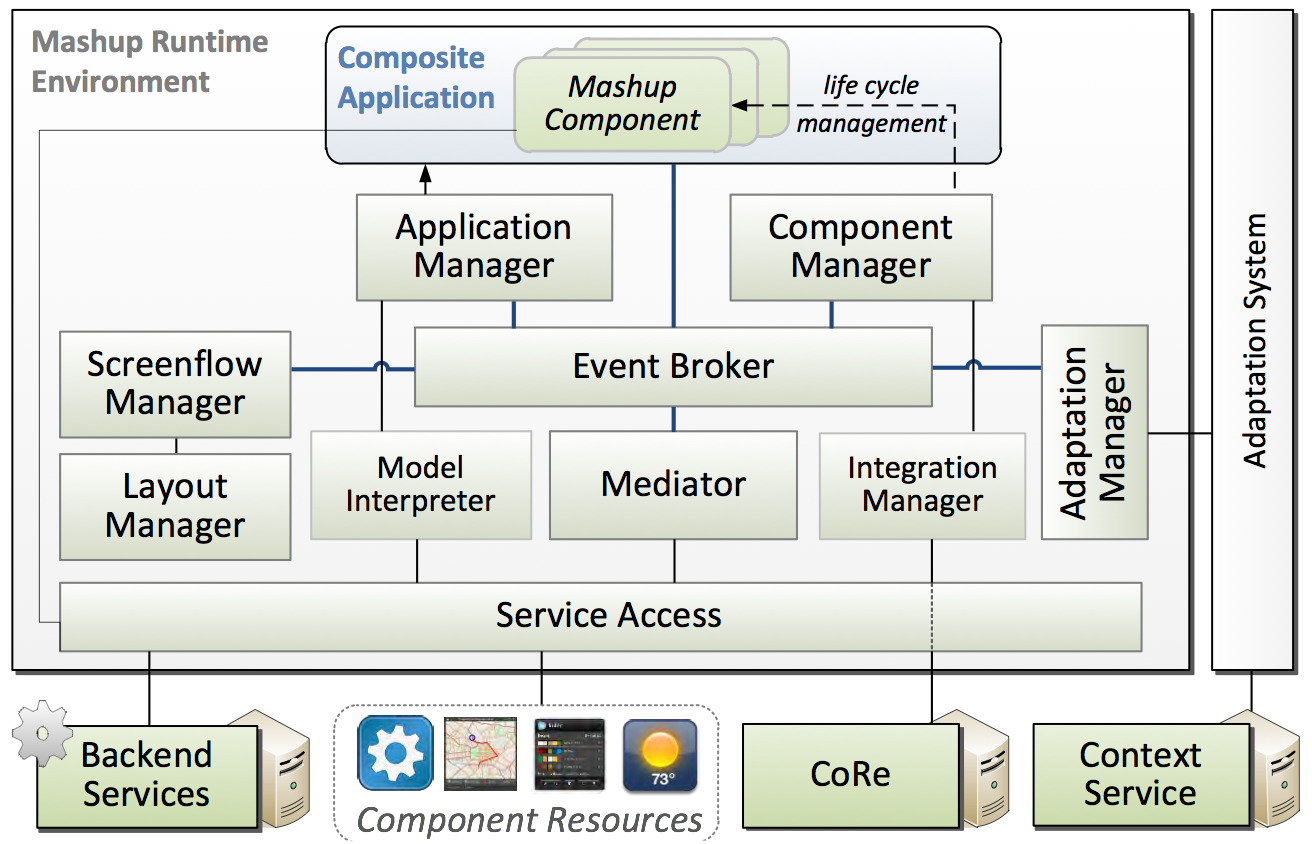
\includegraphics[width=0.75\textwidth]{images/grundlagen-cruise_architektur.png}
	\caption{CRUISe Architektur aus \cite{Pietschmann2012}}
	\label{figure:cruise_architektur}
\end{figure}

CRUISe geht davon aus, dass professionelle Softwarentwickler Komponenten zu kompositen Sichten modellieren, welche dann von Endnutzern nur noch aufgerufen werden. EDYRA \cite{Ruempel2011} greift auf das CRUISe Framework zurück um es Endnutzern selbst zu ermöglichen, diese Aufgabe auszuführen. Dazu schlägt EDYRA zur Laufzeit Komponenten vor, welche sofort integriert oder gelöscht werden können.

VizBoard \cite{Voigt2012} benutzt das CRUISe Framework um Endnutzern die Möglichkeit zu geben, semantische Datensätze mit Hilfe verschiedener InfoVis verstehen zu können. Abbildung~\ref{figure:vizboard_architektur} zeigt die Architektur von VizBoard. Die Daten werden zuerst aus verschiedenen Quellen in eine semantische Repräsentation konvertiert und im Data Repository (DaRe, 1) gespeichert. Das Component Repository (Core, 3) verwaltet die verschiedenen Visualisierungskomponenten (2) und ist für Matching und Ranking von Komponenten zuständig, bevor sie in der Runtime (4) integriert werden. Sowohl das DaRe als auch das CoRe greifen auf die Visualization Ontology (VISO, 5) zurück, die Wissen über verschiedene Aspekte von Visualisierungen, wie z.\,B. Struktur der visualisierten Daten, Mapping der Daten auf visuelle Attribute oder Interaktionsmöglichkeiten, enthält \cite{Voigt2011}.
% architekturbild --> vizboard paper

\begin{figure}[htbp]
	\centering
	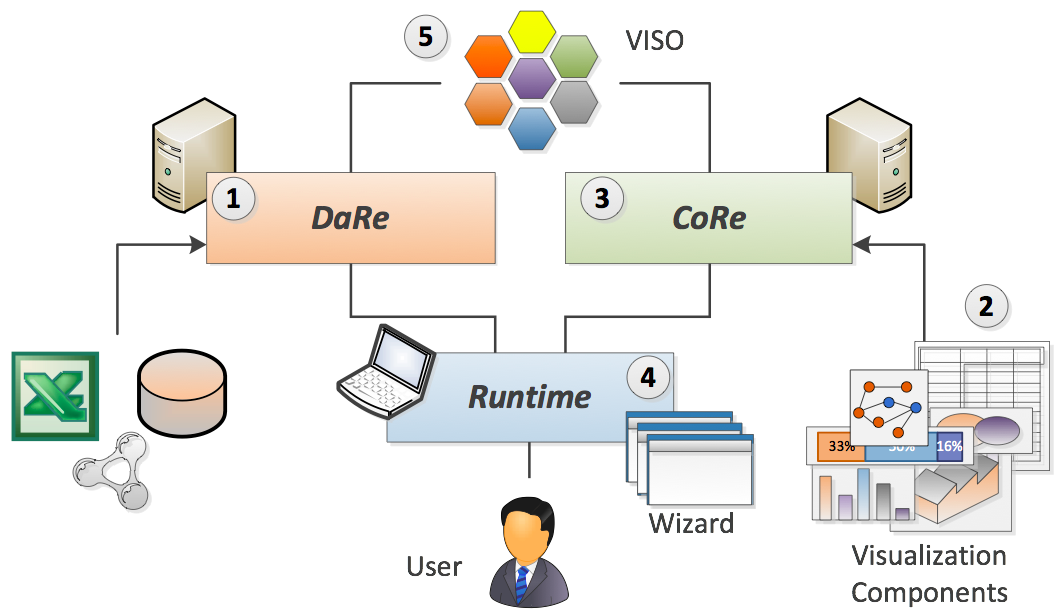
\includegraphics[width=0.75\textwidth]{images/grundlagen-vizboard_architektur.png}
	\caption{VizBoard Architektur aus \cite{Voigt2012}}
	\label{figure:vizboard_architektur}
\end{figure}

\subsubsection{Data Repository}
\label{section:data_repository}

% dare --> vizboard paper, beleg
Im Data Repository (DaRe) werden Daten aus verschiedenen Quellen in einer semantischen Repräsentation gespeichert. Dabei durchläuft das DaRe verschiedene Phasen (Abbildung~\ref{figure:dare_phasen}). Zuerst wird der Datensatz \emph{analysiert} und Metainformationen gesammelt, beispielsweise werden Subklassen gezählt und wichtige Konzepte identifiziert. Diese werden an den Datensatz \emph{annotiert}. Zur Laufzeit müssen diese Erkenntnisse wieder aus dem Datensatz \emph{extrahiert} werden. Das DaRe stellt eine REST API zur Verfügung, über die ein Datensatz abgerufen werden kann.

\begin{figure}[htbp]
	\centering
	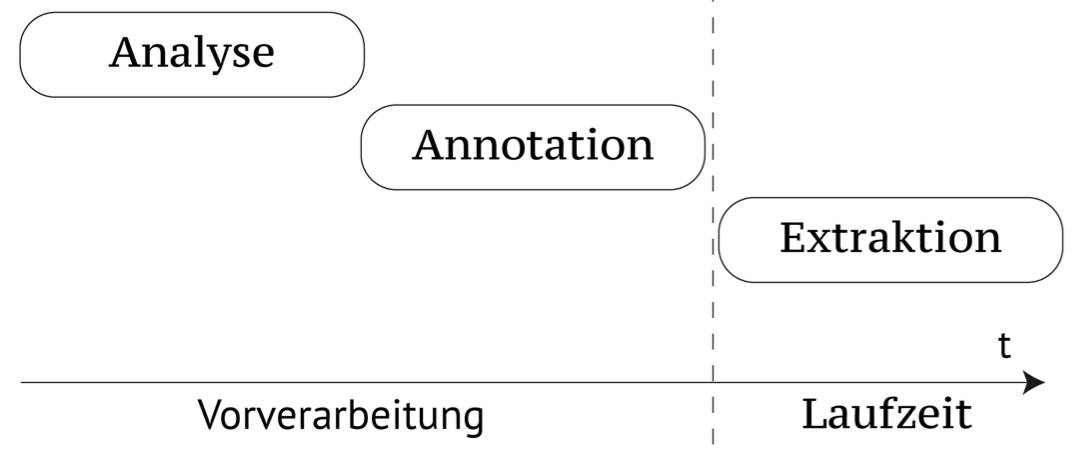
\includegraphics[width=0.5\textwidth]{images/grundlagen-dare_phasen.png}
	\caption{Die Phasen des Data Repository aus \cite{Piccolotto2012}}
	\label{figure:dare_phasen}
\end{figure}

\subsubsection{Komponentenbeschreibung}
\label{section:komponentenbeschreibung}

% komponentenbeschreibung 5.1.3
Komponenten in CRUISe werden generisch und einheitlich durch Properties, Events und Operationen sowie Metainformationen beschrieben. Properties geben Auskunft über den Zustand einer Komponente, also beispielsweise Breite und Höhe oder die Sortierreihenfolge der Elemente. Events weisen andere Komponenten auf interne Zustandsänderungen hin, zum Beispiel wenn sich die Sortierreihenfolge geändert hat. Operationen sind Methoden einer Komponente, die durch Events ausgelöst werden, z.\,B. \texttt{reassignNumbers(order)} um die Nummerierung der Pins in einer Karte anzupassen. Zu den Metainformationen gehören u.\,a. der Name einer Komponente oder der Preis.

\subsubsection{Kommunikationsmodell}
\label{section:kommunikationsmodell}

% kommunikationsmodell 5.2.2
Die Kommunikation von Komponenten untereinander ist ereignisgesteuert, d.\,h. eine Komponente veröffentlicht ein Event, dessen Nachricht mit Hilfe des Publish/Subscribe Paradigma an alle Subscriber in diesem Kanal (Link) übertragen wird. Subscriber reagieren auf das Event indem sie bestimmte Operationen ausführen. Die Übertragung der Nachrichten wird durch sogenannte Links umgesetzt, welche $n$ Events mit $m$ Operationen verbinden. Spezielle Links sind Backlinks, die eine Zweiwegekommunikation zwischen Komponenten ermöglichen und PropertyLinks, die Properties synchron halten. Ein Überblick über die verschiedenen Links ist in Abbildung~\ref{figure:cruise_links} zu sehen.

\begin{figure}[htbp]
	\centering
	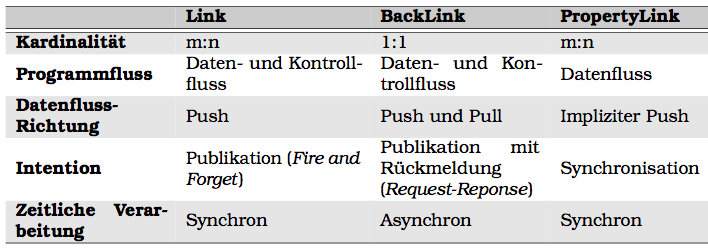
\includegraphics[width=0.75\textwidth]{images/grundlagen-cruise_links.png}
	\caption{CRUISe Links aus \cite{Pietschmann2012}}
	\label{figure:cruise_links}
\end{figure}

\subsubsection{Laufzeitumgebung}
\label{section:laufzeitumgebung}

Die Laufzeitumgebung (Mashup Runtime Environment, MRE) ist für die Ausführung und Verwaltung der kompositen Anwendung verantwortlich und besteht aus mehreren Modulen (Abbildung~\ref{figure:cruise_mre}).

% laufzeitumgebung (tsr) 6.2, 7.2.2
\begin{figure}[htbp]
	\centering
	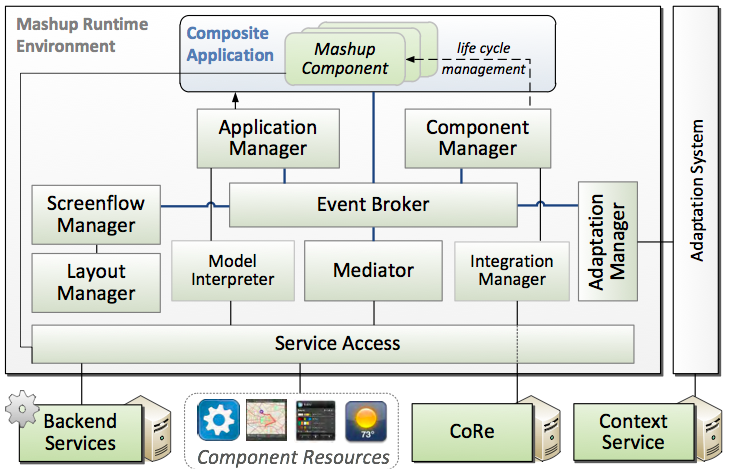
\includegraphics[width=0.75\textwidth]{images/grundlagen-cruise_mre.png}
	\caption{Mashup Runtime Environment Architektur aus \cite{Pietschmann2012}}
	\label{figure:cruise_mre}
\end{figure}

Der \textbf{Application Manager} initialisiert alle anderen Module und ist für die globale Fehlerbehandlung zuständig. Für den Lebenszyklus der einzelnen Komponenten ist der \textbf{Component Manager} zuständig. Die Integration übernimmt allerdings der \textbf{Integration Manager}. Im Mashup Modell definierte Sichten und Übergänge zwischen ihnen werden vom \textbf{Screenflow Manager} interpretiert. Gerendert werden die Komponenten aber vom \textbf{Layout Manager}. Nachrichten zwischen Komponenten der Anwendung und Modulen der MRE werden durch den \textbf{Event Broker} übermittelt. Sind die Parameter von Event und Operation syntaktisch nicht äquivalent, aber semantisch aufeinander abbildbar (z.\,B. zwei gleiche Konzepte aus verschiedenen Namespaces wie \texttt{dbpedia:city} und \texttt{geonames:city}), übernimmt dies der \textbf{Mediator}. Die dynamische Anpassung der Anwendung (z.\,B. von Komponenten, Layout und Kommunikationsmodell) wird gegebenenfalls durch den \textbf{Adaptation Manager} durchgeführt. Letztlich erlaubt das \textbf{Service Access} Modul Zugriff auf Web-Dienste und Ressourcen im Backend.

\subsubsection{VISO}
\label{section:viso}

% viso
In der Visualization Ontology (VISO) ist Visualisierungswissen gespeichert. Sie kann dabei helfen, zur Laufzeit die Domäne dargestellter Daten zu identifizieren oder notwendiges Wissen zur User Assistance (Abschnitt~\ref{section:user_assistance}) zur Komponentenbeschreibung hinzuzufügen. Unter anderem enthält sie folgende Konzepte und deren Verbindungen untereinander:

\begin{itemize}
	\item Visualisierte Daten (\texttt{viso:data})
	\begin{itemize}
		\item Scale of Measurement (nominal, ordinal, quantitativ, unstrukturiert)
		\item Struktur der Daten (tabellarisch, Tripel, verlinkt)
		\item Art der Variable (abhängig, unabhängig, Dimension etc.)
		\item Domäne
	\end{itemize}
	\item Aktivitäten (\texttt{viso:activity})
	\begin{itemize}
		\item Nutzeraktivitäten (Operationen, Aktionen, Aufgaben)
		\item Visualisierungspipeline (Editieren, Visual Mapping, Datentransformation etc.)
	\end{itemize}
	\item Visualisierungen (\texttt{viso:graphic})
	\begin{itemize}
		\item Visuelle Attribute (Größe, Farbe, Textur etc.)
		\item Koordinaten (kartesisch, Zylinder, Kugel etc.)
		\item Charts (Karten, Chart mit zwei Achsen, animierte InfoVis etc.)
		\item Beziehungen zwischen Objekten (Clustering, Labeling, verlinkt etc.)
	\end{itemize}
	\item System (\texttt{viso:system})
	\begin{itemize}
		\item Hardware
		\item Software
		\item Bildschirmauflösung
		\item Rundes, eckiges oder unstrukturiertes Display
	\end{itemize}
\end{itemize}

Dieses Wissen wird in VizBoard auf verschiedene Art und Weise genutzt (Abbildung~\ref{figure:viso}). Mit Hilfe der VISO kann Wissen von Visualisierungsexperten formalisiert und im Rankingalgorithmus berücksichtigt werden (2). Gleichermaßen wird sie zur Annotation der Daten im Data Repository (Abschnitt~\ref{section:data_repository}) benutzt (3). Visualisierungskomponenten (4) und Nutzer- bzw. Systemkontext (5) werden durch VISO-Konzepte beschrieben.

\begin{figure}[htbp]
	\centering
	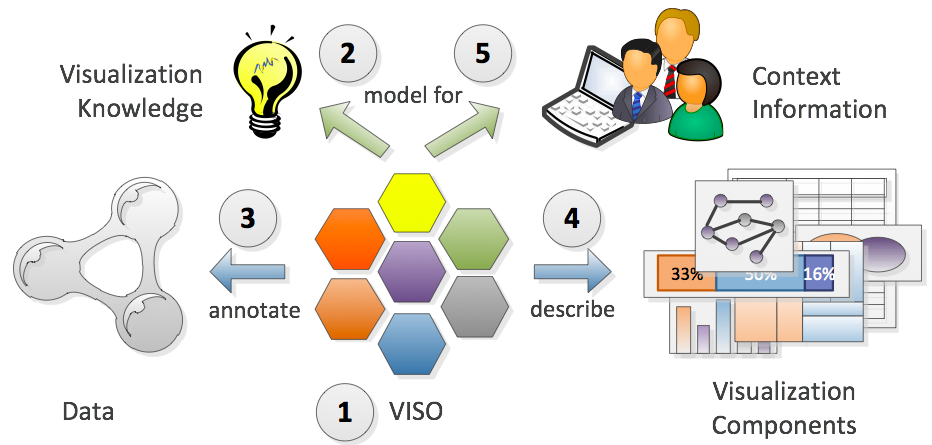
\includegraphics[width=0.75\textwidth]{images/grundlagen-viso.png}
	\caption{Nutzung der VISO in VizBoard}
	\label{figure:viso}
\end{figure}

\subsection{Semantische Datensätze}
\label{section:semantische_daten}

% Grundlagen von RDF, RDFS, OWL. Wichtig weil später Kommentare wieder in einer Ontologie abgelegt werden müssen
Eine Ontologie ist \enquote{an explicit specification of a conceptualization} \cite{Gruber1995} und wird benutzt um domänenspezifisches Wissen abzubilden \cite{Chandrasekaran1999}. Sie besteht aus mehreren Elementen:

\begin{itemize}
	\item Eine Klasse repräsentiert ein Konzept, eine Entität, ein Ding, beispielsweise ein \textit{Smartphone}.
	\item Eine Instanz ist ein konkretes Objekt einer Klasse, zum Beispiel das \textit{iPhone mit der Seriennummer XYZ-ABC}.
	\item Datenattribute beschreiben eine Instanz näher, zum Beispiel die \textit{Seriennummer} oder \textit{Bildschirmgröße} des iPhones.
	\item Objektattribute beschreiben Beziehungen zwischen Klassen und deren Instanzen, beispielsweise eine Person \textit{besitzt} ein Smartphone.
	\item Außerdem existieren noch Axiome, Regeln, Funktionen und Einschränkungen, welche die Logik einer Ontologie beschreiben.
\end{itemize}

Um eine Ontologie maschinenlesbar darzustellen, hat das World Wide Web Consortium (W3C) verschiedene Beschreibungssprachen eingeführt. Die bekanntesten sind Resource Description Framework Schema (RDFS) und Web Ontology Language (OWL). Mit diesen Sprachen lässt sich unterschiedlich viel Semantik u.\,a. in Form von Ontologien, Thesauren oder Vokabularen ausdrücken; die Komplexität der Dokumente und damit der Aufwand, sie zu erstellen, verhalten sich aber direkt proportional (siehe Abbildung~\ref{figure:semantic_spectrum}).

\begin{figure}[htbp]
	\centering
	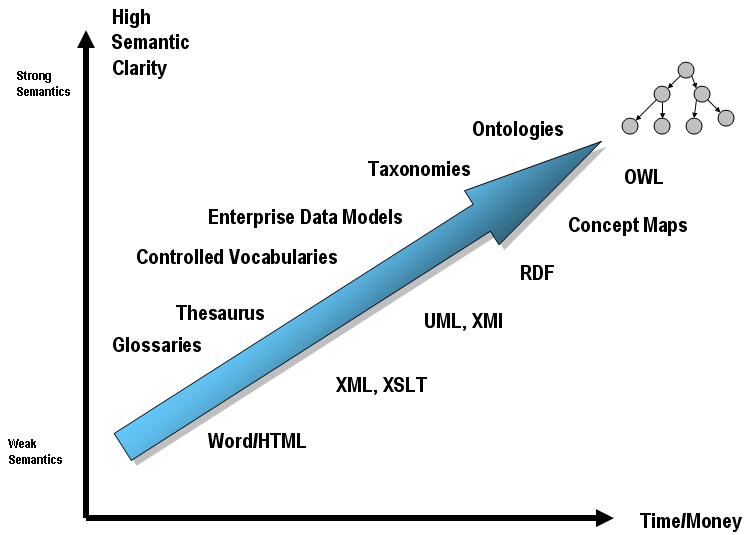
\includegraphics[width=0.75\textwidth]{images/grundlagen-semantic_spectrum.png}
	\caption{Semantic Spectrum \cite{Bergman2007}}
	\label{figure:semantic_spectrum}
\end{figure}

Sprache mit wenigsten Features, aber sehr verbreitet: RDF, hier nur Tripel der Form (S, P, O).

Klassen und andere Schemainformationen mit RDFS.

OWL bringt dann Konzepte aus der Logik wie Axiome und Funktionen.

Mächtigkeit: RDF < RDFS < OWL

\subsection{Informationsvisualisierung}
\label{section:informationsvisualisierung}

% InfoVis Grundlagen. Wichtig weil das die Komponenten sind, mit denen ich zu tun habe.

Card et al. \cite{Card1999} definieren den Begriff \enquote{Informationsvisualisierung} wie folgt:

\begin{quote}
The use of computer-supported, interactive, visual representations of abstract data to amplify cognition.
\end{quote}

Beispiele dafür sind Balkendiagramme, Treemaps \cite{Shneiderman1992} und Parallel Coordinates \cite{Inselberg1991} (Abbildung~\ref{figure:parallel_coordinates}). Mangels Interaktivität sind Infografiken \cite{Smiciklas2012} von den eben definierten Informationsvisualisierungen ausgeschlossen.

\begin{figure}[htbp]
   \centering
   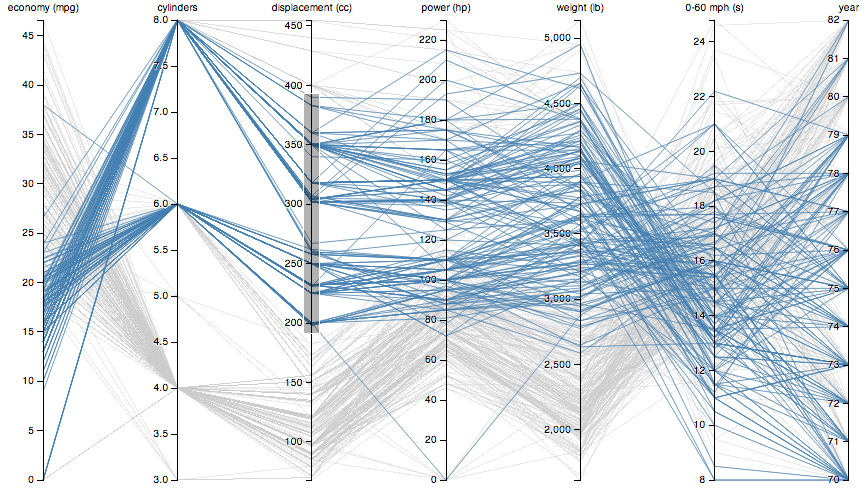
\includegraphics[width=0.5\textwidth]{images/grundlagen-parallel_coordinates.png} 
   \caption{Parallel Coordinates}
   \label{figure:parallel_coordinates}
\end{figure}

Informationsvisualisierungen können besonders bei der Exploration großer Datenmengen hilfreich sein \cite{Kohlhammer2011}. Die Wissensaneignung erfolgt dabei iterativ (Abbildung~\ref{figure:visual_analytics_process}). Zuerst werden Daten auf eine Visualisierung gemappt, deren Parameter vom Benutzer geändert werden können. Daraus lernt dieser etwas über die Daten und kann danach (\enquote{Feedback loop}) von vorne anfangen und eine andere Visualisierung wählen oder die Daten transformieren.

\begin{figure}[htbp]
   \centering
   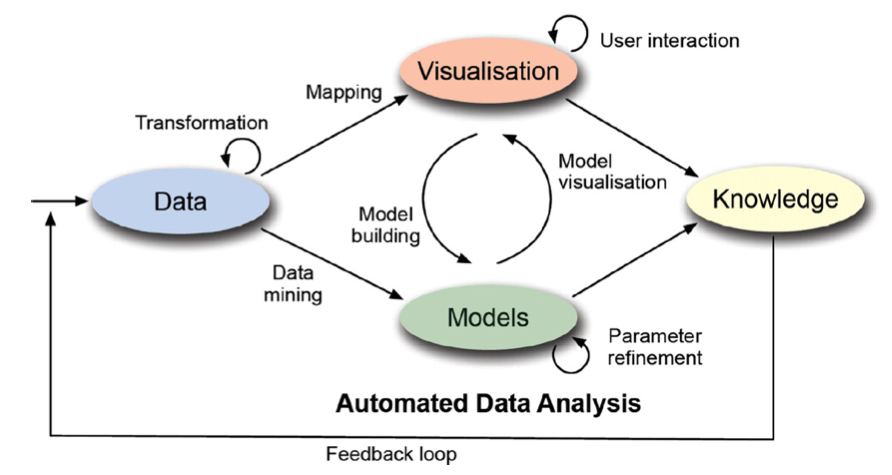
\includegraphics[width=0.5\textwidth]{images/grundlagen-visual_analytics_process.png} 
   \caption{Visual Analytics Process nach \cite{Kohlhammer2011}}
   \label{figure:visual_analytics_process}
\end{figure}

Van Wijk \cite{vanWijk2005} stellt ein ähnliches Modell für den Prozess der Wissensaufnahme über Visualisierungen vor (Abbildung~\ref{figure:visualization_model}). Am Anfang stehen die Daten $D$, welche anhand einer Visualisierungsspezifikation $S$ in eine Visualisierung $V$ transformiert werden. Diese wird vom Benutzer aufgenommen ($P$) und in Wissen ($K$) umgesetzt. Danach startet die Exploration der Daten $E$ indem die Spezifikation geändert und neues Wissen aufgenommen wird (entspricht der \enquote{Feedback loop} aus \cite{Kohlhammer2011}).

\begin{figure}[htbp]
   \centering
   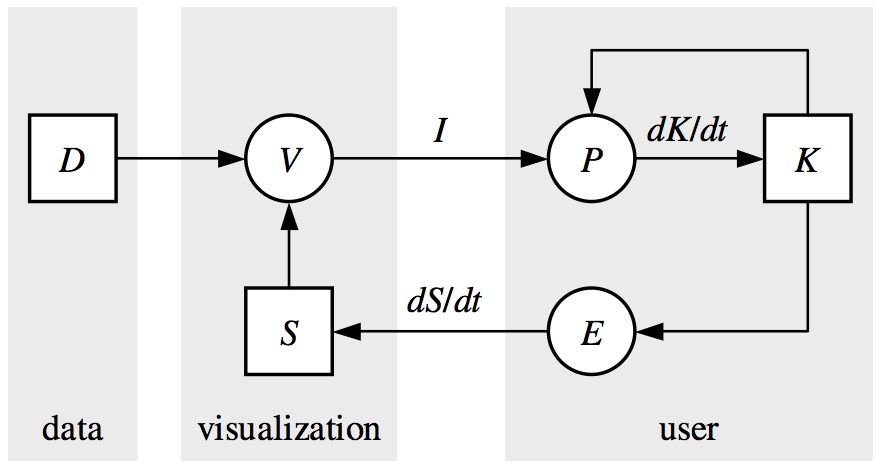
\includegraphics[width=0.5\textwidth]{images/grundlagen-visualization_model.png} 
   \caption{Generic Model on Visualization nach \cite{vanWijk2005}}
   \label{figure:visualization_model}
\end{figure}

Im Folgenden wird ein Überblick über verschiedene Informationsvisualisierungen gegeben. Dieser orientiert sich an Keim \cite{Keim2002}, welcher Informationsvisualisierungen nach dargestellten Daten, Visualisierungs- und Interaktionstechnik klassifizierte. Die Abbildungen stammen, sofern nicht anders angegeben, aus \cite{Heer2010}.

\subsubsection{Dargestellte Daten}
\label{section:dargestellte_daten}

\textbf{Eindimensionale Daten} sind beispielsweise Zeitreihen, also Folgen von Daten (1992, 1993, 1995...). Nach Keim können diese aber mit anderen Datenobjekten assoziiert sein. Beispiele für InfoVis eindimensionaler Daten wären demnach ein Index Chart (Abbildung~\ref{figure:index_chart}) oder eine einfache Timeline.

\begin{figure}[htbp]
   \centering
   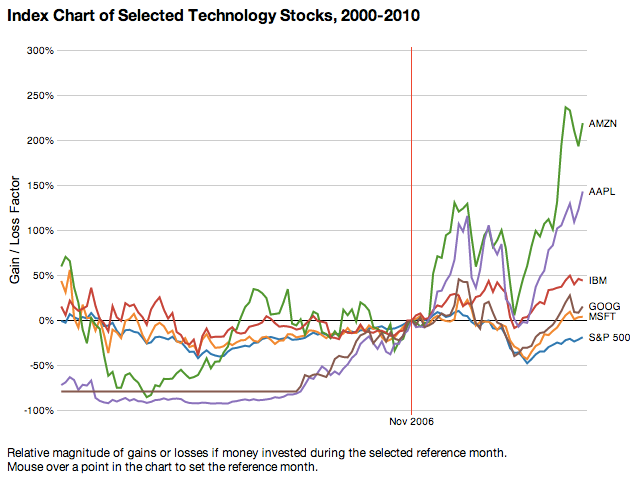
\includegraphics[width=0.5\textwidth]{images/grundlagen-index_chart.png}
   \caption{Index Chart}
   \label{figure:index_chart}
\end{figure}

\textbf{Zweidimensionale Daten} haben zwei unterschiedliche Dimensionen, wie zum Beispiel eine Geokoordinate (geografische Länge und Breite). Beispiele für InfoVis dieser Daten sind eben Karten (Abbildung~\ref{figure:karte}) oder häufig verwendete zweidimensionale Visualisierungen wie z.\,B. ein Balkendiagramm.

\begin{figure}[htbp]
   \centering
   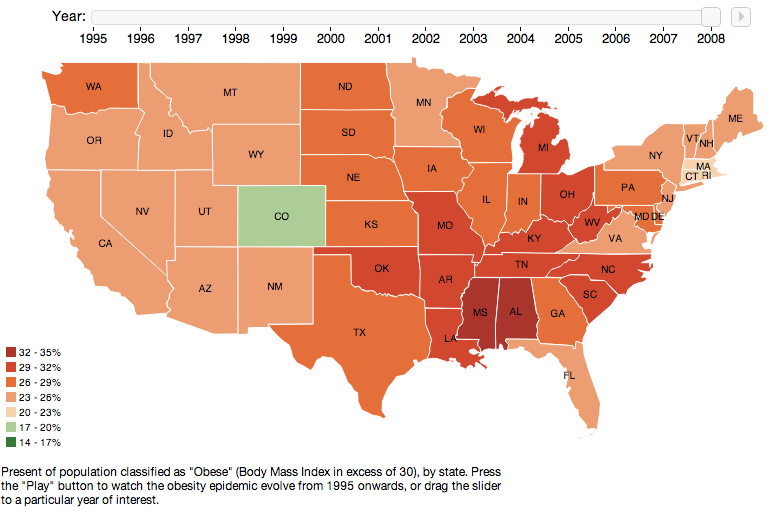
\includegraphics[width=0.5\textwidth]{images/grundlagen-karte.png}
   \caption{Karte}
   \label{figure:karte}
\end{figure}

\textbf{Multidimensionale Daten} haben demnach mehr als zwei unterschiedliche Dimensionen, typischerweise komplexe Objekte wie Autos (Hubraum, Maximalgeschwindigkeit, Leistung, Benzinverbrauch...) oder Digitalkameras (Megapixel, Sensorgröße, maximale Lichtempfindlichkeit, Gewicht...). Um diese Daten darzustellen, werden oft Parallel Coordinates (Abbildung~\ref{figure:parallel_coordinates}) oder Scatterplot Matrizen (Abbildung~\ref{figure:scatterplot_matrix}) verwendet.

\begin{figure}[htbp]
   \centering
   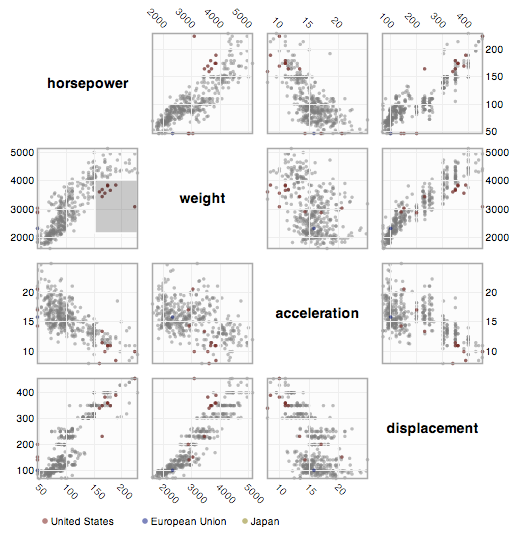
\includegraphics[width=0.5\textwidth]{images/grundlagen-scatterplot_matrix.png}
   \caption{Scatterplot Matrix}
   \label{figure:scatterplot_matrix}
\end{figure}

\textbf{Text} kann erst nach einer Vorverarbeitungsphase mit Zahlen beschrieben werden (z.\,B. Wörter zählen), ansonsten schlagen herkömmliche Visualisierungsansätze fehl. Ein im Web verbreitetes Beispiel ist die Tag Cloud (Abbildung~\ref{figure:tag_cloud}\footnote{\url{http://4.bp.blogspot.com/-WvicpJ9QqQs/TpbqvbKhX3I/AAAAAAAADGc/3PczLY2P0xs/s1600/uni_tag_cloud_wordle.png}}). Je häufiger ein Begriff im Textkorpus vorkommt, desto größer wird er dargestellt.

\begin{figure}[htbp]
   \centering
   
\includegraphics[width=0.5\textwidth]{images/grundlagen-tag_cloud.png}
   \caption{Tag Cloud}
   \label{figure:tag_cloud}
\end{figure}

\textbf{Hierarchien und Netzwerke} beschreiben Relationen und Verbindungen zwischen Objekten. Ein Beispiel für InfoVis von Hierarchien ist der klassische Baum (Abbildung~\ref{figure:baum}), für Netzwerke ein Node-Link-Diagramm (Abbildung~\ref{figure:node-link-diagramm}).

\begin{figure}[htbp]
   \centering
   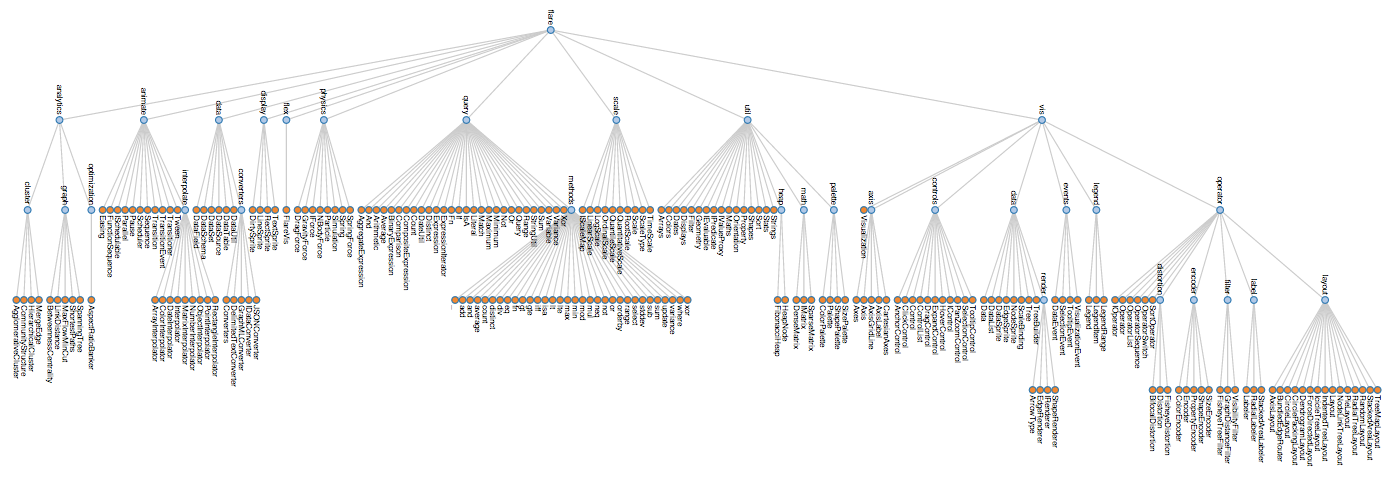
\includegraphics[width=0.75\textwidth]{images/grundlagen-baum.png}
   \caption{Baum}
   \label{figure:baum}
\end{figure}

\begin{figure}[htbp]
   \centering
   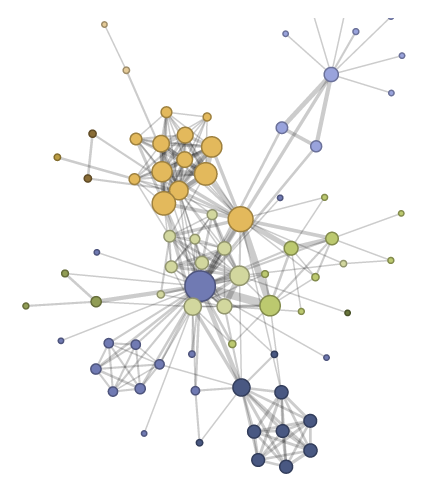
\includegraphics[width=0.25\textwidth]{images/grundlagen-node-link-diagramm.png}
   \caption{Node-Link-Diagramm}
   \label{figure:node-link-diagramm}
\end{figure}

% Am Schluss hat Keim noch Software/Algorithmen, aber ich sehe den Unterschied zu Multidimensionalen Daten nicht. Außerdem kann man - wenn schon mal grundlos neue Kategorien eingeführt werden - dann auch Produktionsprozesse oder what not gesondert betrachten

\subsubsection{Visualisierungstechniken}
\label{section:Visualisierungstechniken}

% standard 2d/3d

\textbf{Standard 2D/3D} Visualisierungen beinhalten Balkendiagramme, Liniendiagramme, sowie andere zweidimensionale Plots und Karten. Ein Beispiel dafür ist das Index Chart (Abbildung~\ref{figure:index_chart}).

% multidimensional
\textbf{Multidimensionale} Visualisierungen\footnote{Die Bezeichnung stammt von Chi \cite{Chi2000} und wird verwendet, da sie logischer erscheint als Keims \enquote{geometrically transformed displays}.} sind Darstellungen multidimensionaler Datensätze jeder Art. Beispiele sind Parallel Coordinates (Abbildung~\ref{figure:parallel_coordinates}) und die Scatterplot Matrix (Abbildung~\ref{figure:scatterplot_matrix}).

% iconic displays

\textbf{Symbolische} Visualisierungen setzen auf verschiedene Art und Weise Symbole ein. Das können auf eine Karte projizierte Kuchendiagramme sein (Abbildung~\ref{figure:symbol_map}) oder Smileys, die abhängig von den Daten lächeln oder weinen \cite{Chernoff1973}.

\begin{figure}[htbp]
   \centering
   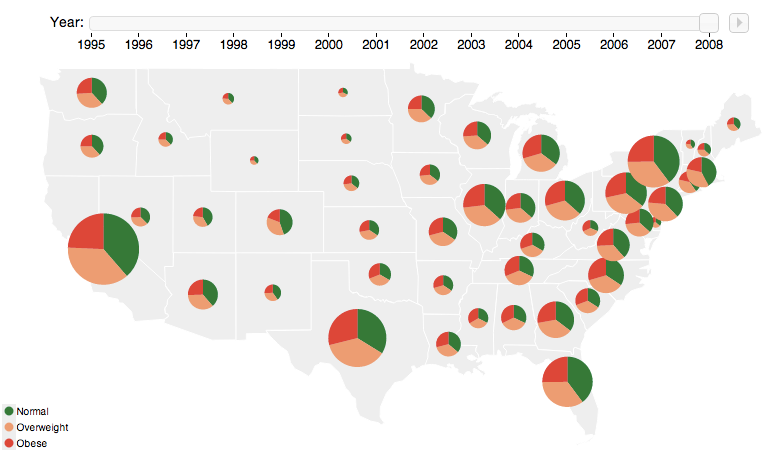
\includegraphics[width=0.5\textwidth]{images/grundlagen-symbol_map.png}
   \caption{Symbol Map}
   \label{figure:symbol_map}
\end{figure}

% dense pixel displays

\textbf{Dense Pixel} Visualisierungen assoziieren jeden Wert einer Dimension mit einem eingefärbten Pixel und platzieren die Pixel einer Dimension nebeneinander. Ein Beispiel dafür ist das Recursive Pattern \cite{Keim1995} (Abbildung~\ref{figure:recursive_pattern}).

\begin{figure}[htbp]
   \centering
   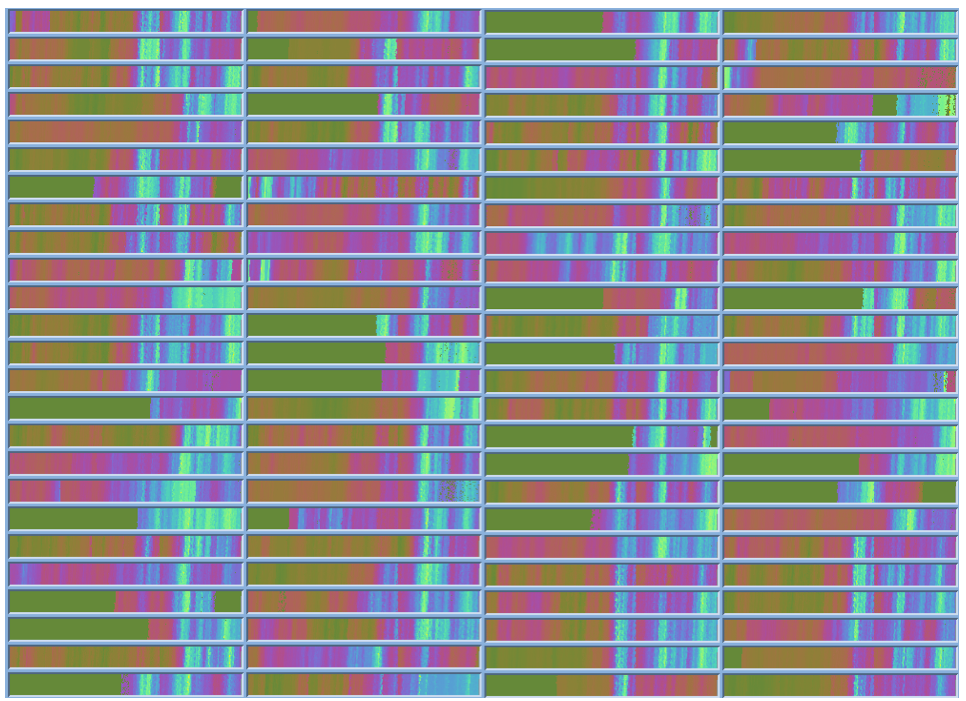
\includegraphics[width=0.5\textwidth]{images/grundlagen-recursive_pattern.png}
   \caption{Recursive Pattern}
   \label{figure:recursive_pattern}
\end{figure}

% stacked displays

\textbf{Verschachtelte} Visualisierungen repräsentieren Hierarchien, wobei Kindknoten innerhalb ihrer Eltern dargestellt werden. Beispiele dafür sind Treemaps \cite{Shneiderman1992} oder Nested Circles (Abbildung~\ref{figure:nested_circles}).

\begin{figure}[htbp]
   \centering
   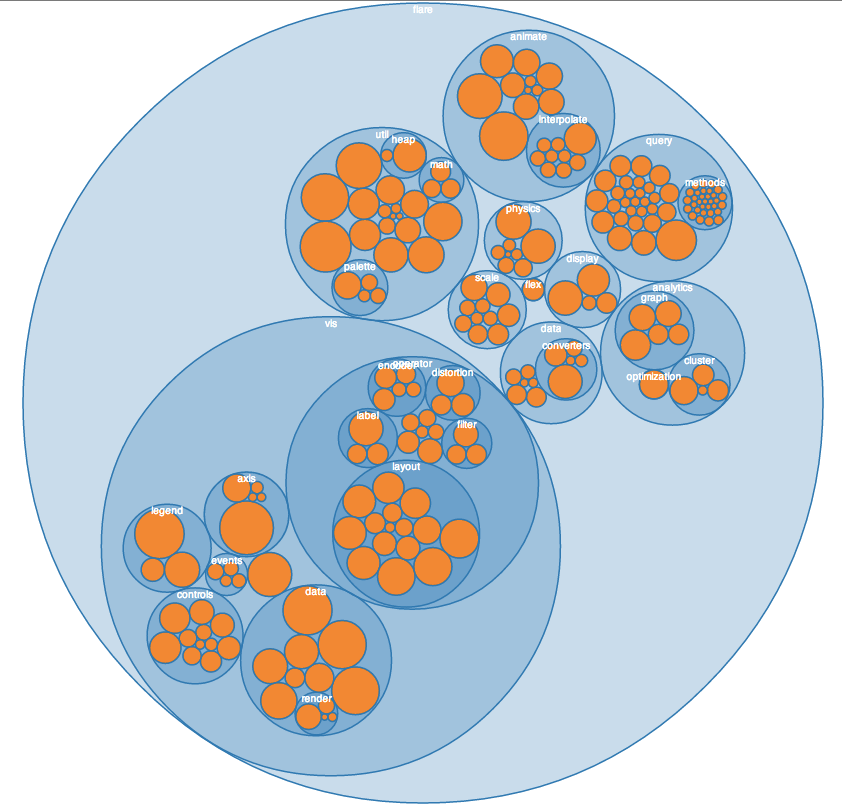
\includegraphics[width=0.25\textwidth]{images/grundlagen-nested_circles.png}
   \caption{Nested Circles}
   \label{figure:nested_circles}
\end{figure}

\subsubsection{Interaktionstechniken}
\label{section:interaktionstechniken}

% dynamische projektionen

\textbf{Dynamische Projektionen} zeigen dem Benutzer automatisch beispielsweise verschiedene Scatterplots des Datensatzes. Diese Interaktionstechnik eignet sich besonders für multidimensionale Datensätze. Umgesetzt wurde sie zum Beispiel in XGobi \cite{Swayne1998}.

% interaktives filtern

Durch \textbf{interaktives Filtern} bestimmt der Benutzer, welche Teilmenge des Datensatzes visualisiert wird. Das kann durch direktes Auswählen (Browsing) oder durch Bestimmen von Eigenschaften der gewünschten Daten (Querying) passieren. Letzteres ist in modernen E-Commerce-Systemen durch Facetten \cite{Yee2003} umgesetzt (Abbildung~\ref{figure:faceted_browsing}).

\begin{figure}[htbp]
   \centering
   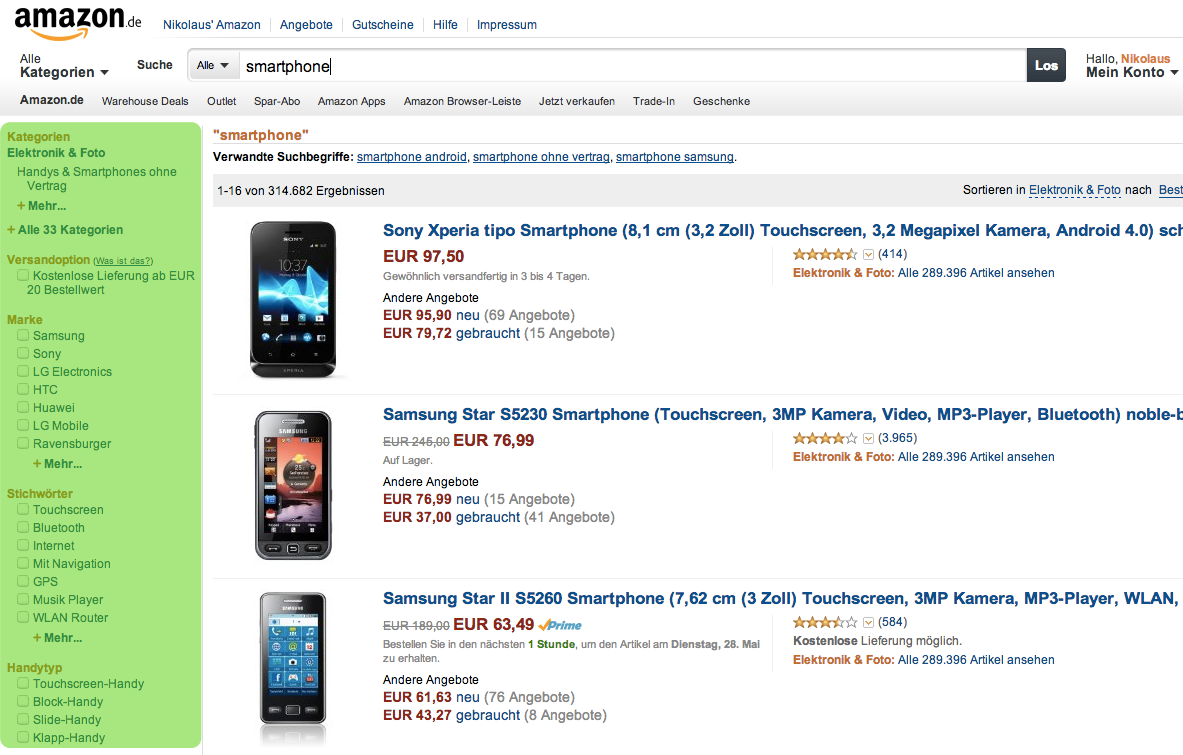
\includegraphics[width=0.5\textwidth]{images/grundlagen-faceted_browsing.png}
   \caption{Faceted Browsing bei Amazon.de}
   \label{figure:faceted_browsing}
\end{figure}

% interaktives zoomen

\textbf{Interaktives Zoomen} ermöglicht es dem Benutzer mehr oder weniger Details anzuzeigen. Damit ist nicht nur der computergrafische Vorgang der Skalierung gemeint (wie etwa bei einem Mikroskop), sondern auch schlecht sichtbare Elemente auszublenden (wie z.\,B. bei Google Maps, siehe Abbildung~\ref{figure:zoom}).

\begin{figure}[htbp]
   \centering
   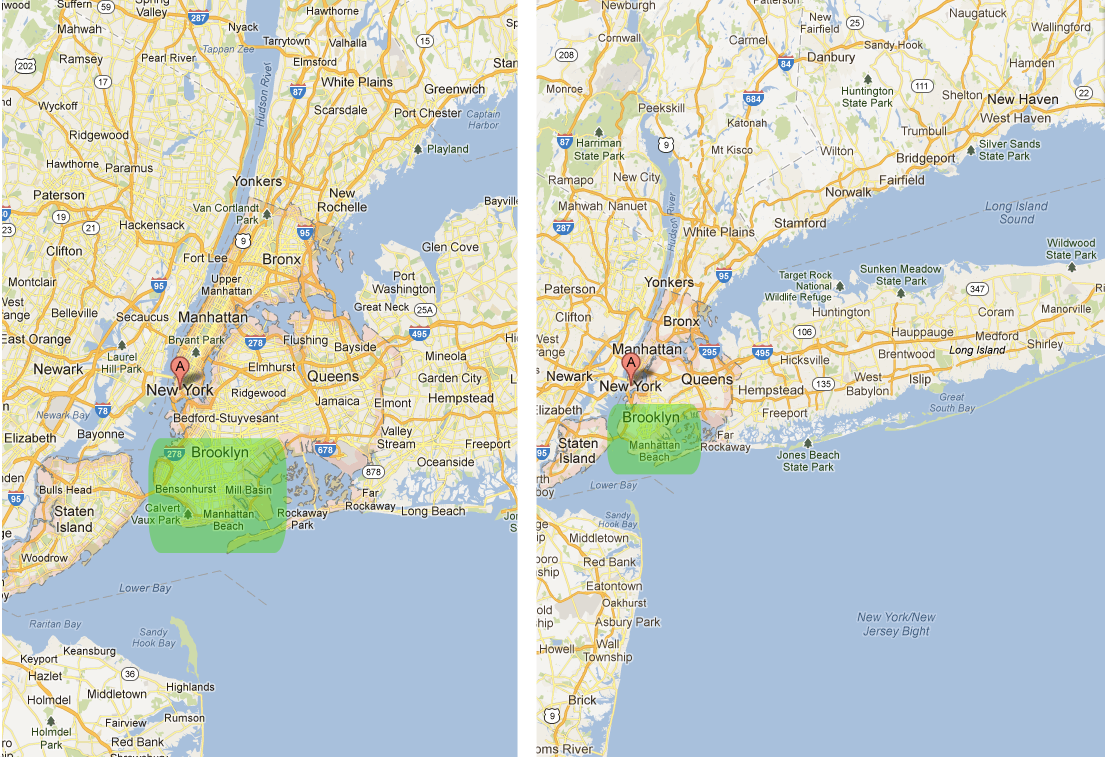
\includegraphics[width=0.5\textwidth]{images/grundlagen-zoom.png}
   \caption{Interaktiver Zoom bei Google Maps: Im rechten, ausgezoomten Bild fehlt beispielsweise die Interstate 278 (grüne Markierung)}
   \label{figure:zoom}
\end{figure}

% distortion (fisheyes and such)

Durch \textbf{Verzerrung} kann ein Bereich der Visualisierung mit hohem Detailgrad angezeigt werden, während der Rest nur wenig detailliert sichtbar ist. Ein bekanntes Beispiel dafür ist das Fisheye (Abbildung~\ref{figure:fisheye}).

\begin{figure}[htbp]
   \centering
   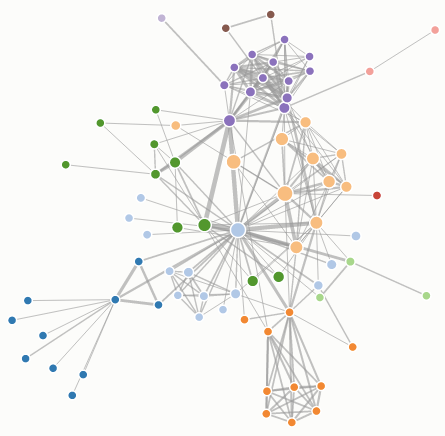
\includegraphics[width=0.5\textwidth]{images/grundlagen-fisheye.png}
   \caption{Fisheye: Das Zentrum der Verzerrung befindet sich ungefähr beim hellblauen Knoten in der Mitte}
   \label{figure:fisheye}
\end{figure}

% link & brush

\textbf{Linking \& Brushing} wird vor allem bei mehreren verschiedenen Visualisierungen eingesetzt. Die in einer Visualisierung markierten Daten werden auch in allen anderen Visualisierungen hervorgehoben. Das können zum Beispiel Scatterplots (siehe multidimensionale Visualisierungen in Abschnitt~\ref{section:Visualisierungstechniken}), verschiedene Histogramme (Abbildung~\ref{figure:link_brush}\footnote{\url{http://square.github.io/crossfilter/}}) oder gemischte Visualisierungen sein.

\begin{figure}[htbp]
   \centering
   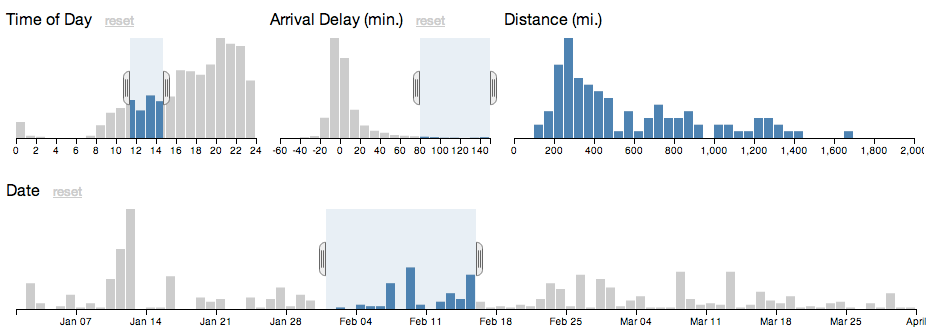
\includegraphics[width=0.75\textwidth]{images/grundlagen-link_brush.png}
   \caption{Linking \& Brushing bei Crossfilter.js: Ausgewählt wurden Flüge mit mehr als 80 Minuten Verspätung, die betroffenen Bereiche in anderen Histogrammen wurden automatisch markiert.}
   \label{figure:link_brush}
\end{figure}

todo: Was habe ich daraus jetzt gelernt?

\subsection{User Assistance}
\label{section:user_assistance}

% was ist assistance?

Der Begriff \enquote{User Assistance} steht für verschiedene Möglichkeiten, einem Benutzer zu helfen seine Ziele zu erreichen. Gapenne et al. \cite{Gapenne2002} definieren vier Beziehungstypen zwischen Mensch und Technologie, welche auch konkret auf Software übertragen werden können. Einer davon ist Assistance:

\begin{quote}
The assistance relationship appears as a sub-category of supplementation since it is not a crucial one for the actual and main activity. The function of this type of technology is to qualify and display the state and/or the becoming of the supplementation device which the subject is engaged in.
\end{quote}

Assistance sind also zum Beispiel eine Einparkhilfe im Auto oder eine Eieruhr in der Küche: Erfolgreiches Einparken oder Kochen ist auch ohne sie möglich, aber leichter mit ihnen. Supplementation hingegen erweitert die Fähigkeiten des Anwenders, also zum Beispiel eine Handprothese mit der die Pfanne angefasst werden kann.

% wie kann man assistance klassifizieren?

Rech et al. \cite{Rech2007} beschreiben intelligente Assistance in der Softwareentwicklung. Prinzipiell müssen zuerst Daten gesammelt werden, bevor die Assistance generiert und angeboten werden kann (Abbildung~\ref{figure:intelligent_assistance}). Folgende Punkte müssen in den einzelnen Schritten beachtet werden.

\begin{itemize}

	\item Daten sammeln
	\begin{itemize}
		\item Welche Datenquellen sollen benutzt werden?
		\item Wann soll die Datenanalyse stattfinden?
		\item Wie können Erkenntnisse aus den Daten gewonnen werden?
	\end{itemize}
	\item Assistance generieren
	\begin{itemize}
		\item Für wen ist die Assistance gedacht?
		\item Was soll durch Assistance erweitert werden?
		\item Für welchen Prozess/Vorgang ist die Assistance gedacht?
		\item Was ist die Zielumgebung der Assistance?
	\end{itemize}
	\item Assistance anbieten
	\begin{itemize}
		\item Wann soll Asssistance angeboten werden?
		\item Welche Modalität (visuell, akustisch usw.) soll die Assistance anbieten?
		\item Wo soll die Information angezeigt werden?
		\item Warum muss dem Benutzer geholfen werden?
	\end{itemize}
\end{itemize}

\begin{figure}[htbp]
   \centering
   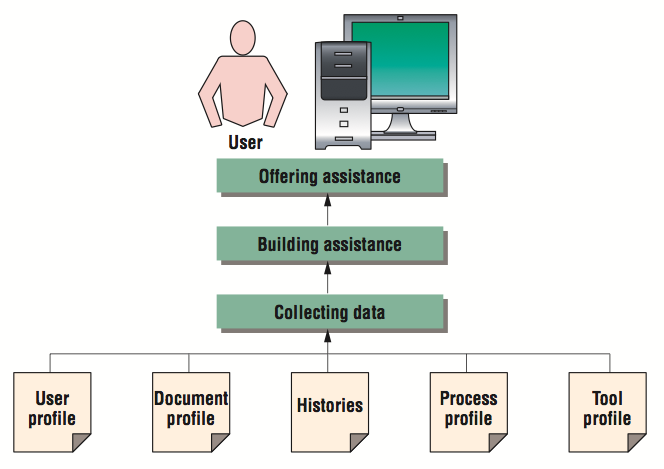
\includegraphics[width=0.5\textwidth]{images/grundlagen-intelligent_assistance.png}
   \caption{Intelligente Assistance nach \cite{Rech2007}}
   \label{figure:intelligent_assistance}
\end{figure}

Besonders die Modalität der Assistance erscheint von großer Bedeutung für eine schnelle und effektive Wissensaufnahme. Wie Information wahrgenommen wird hat Auswirkungen sowohl auf Verständnis (\enquote{Ein Bild sagt mehr als tausend Worte}) als auch auf die benötigte Zeit. Tausend Worte können auf der Suche nach relevanten Informationen immer noch überflogen werden, eine zehnminütige akustische Hilfestellung nicht.

% effektivität von textuellen, akustischen, visuellen, gemischten erklärungen

Da kein Medium (Film, Audio, Buch etc.) besser zum Lernen geeignet ist als ein anderes \cite{Clark1994, Kozma1994} und multimodale Erklärungen effektiver als monomodale sind \cite{Mayer2002}, stellt sich die Frage, wie Multimedia-Hilfe konstruiert werden soll. Dazu kann auf die kognitive Multimedia-Lerntheorie zurückgegriffen werden. Sie geht davon aus, dass Menschen Wissen grundsätzlich über zwei Kanäle (visuell und verbal) aufnehmen, entsprechende Repräsentationen bilden und mit vorhandenem Wissen verknüpfen (Abbildung~\ref{figure:kognitive_multimedia_lerntheorie}). Die beiden Aufnahmekanäle sind in ihrer Kapazität beschränkt. Müssen zu viele Informationen verarbeitet werden, kommt es zum \enquote{Cognitive Overload} und die Lernfähigkeit wird eingeschränkt. Daraus ergeben sich vier Richtlinien zur Kontruktion der Multimedia-Erklärungen:

\begin{itemize}
	\item \textbf{Gleichzeitigkeit}: Werden akustische und visuelle Mittel eingesetzt, so sollen sie gleichzeitig präsentiert werden \cite{Mayer1991}. So können Lernende ihre visuellen und verbalen Wissensrepräsentationen besser miteinander verknüpfen.
	\item \textbf{Prägnanz}: Unterhaltsame aber irrelevante Details fördern die Erinnerungsfähigkeit an einen Text nicht \cite{Garner1989}. Deswegen sollen nur relevante Informationen vermittelt werden.
	\item \textbf{Multimodalität}: Informationen sollten möglichst auf visuelle und verbale Art vermittelt werden, um zu verhindern, dass ein Aufnahmekanal überlastet wird (bspw. durch die Darstellung einer Animation mit On-Screen-Text) \cite{Moreno1999}.
	\item \textbf{Keine Redundanz}: Aus dem selben Grund warum zweikanälige Erklärungen vorzuziehen sind, sollte auch Redundanz in einem Aufnahmekanel vermieden werden.
\end{itemize}

\begin{figure}[htbp]
   \centering
   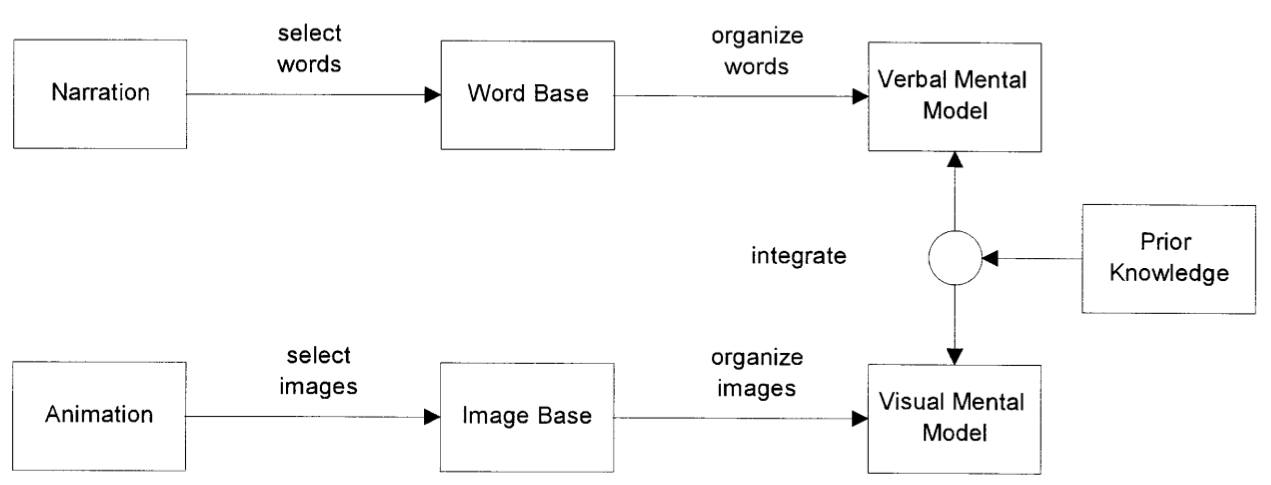
\includegraphics[width=0.75\textwidth]{images/grundlagen-kognitive_multimedia_lerntheorie.png}
   \caption{Kognitive Multimedia-Lerntheorie nach \cite{Mayer2002}}
   \label{figure:kognitive_multimedia_lerntheorie}
\end{figure}

% user assistance möglichkeiten für jede modalität

Wie kann User Assistance im visuellen bzw. verbalen Aufnahmekanal aussehen? Verbale Erklärungen können zur Laufzeit generiert werden \cite{Bauer2011, Gesell2012, Matheson2012}, sind jedoch tendenziell zu langatmig formuliert und enthalten viele Wiederholungen. Auf Grund der vorhin erwähnten Designprinzipien \enquote{Prägnanz} und \enquote{Keine Redundanz} sollte davon wahrscheinlich abgesehen und verbale Erklärungen handgeschrieben oder sehr kurz gehalten werden.

Die naheliegendste Möglichkeit für visuelle User Assistance sind Bilder. Illustrationen/Schemata sind in der Tat hilfreich, solange sowohl die Bestandteile des Systems (z.\,B. eine Luftpumpe) als auch die einzelnen Schritte des Prozesses (z.\,B. pumpen) dargestellt werden \cite{Mayer1990}. Auch Comics sind gut geeignet um Sachverhalte zu erklären (siehe z.\,B. \cite{McCloud1994, McCloud2008}) und eine ansprechende Variante für User Assistance \cite{Webb2012}.

Animationen im Sinne von kurzen Videos mit abstrahiertem Inhalt können ebenfalls ein geeigneter Weg sein um Wissen zu vermitteln, sofern die erwähnten Designprinzipien eingehalten werden \cite{Mayer2002a}. Allerdings ist es möglich, dass Benutzer mit wenig Vorwissen weniger davon profitieren also solche mit viel Vorwissen \cite{Kalyuga2008}. Wenn Animationen eingesetzt werden, sollte den Benutzern Kontrolle über die Geschwindigkeit der Animation gegeben und wichtige Teile gekennzeichnet werden \cite{Wong2011}. Bei Web User Interfaces besteht die Möglichkeit konkrete Elemente der InfoVis für die Animation heranzuziehen. Das würde dem Prinzip der \enquote{Semantic Transparency} \cite{Kohlhase2009} entsprechen, wonach Benutzer möglichst direkt auf den für ihre Ziele relevanten UI-Elementen arbeiten sollen.

Filme? Hier gibt es eine Doktorarbeit, aber die finde ich online nicht \url{http://search.proquest.com/docview/1286857518}. Ansonsten scheint sich damit niemand so richtig zu beschäftigen und eigentlich ist es mir auch wurscht weil Tutorialvideos einen immer so aus dem Arbeitskontext reissen.


\subsubsection{Sensemaking}
\label{section:sensemaking}

% was ist der unterschied zwischen learning und sensemaking?
Im vorhergehenden Abschnitt wurde der Prozess der Wissensvermittlung betrachtet. Um Wissen dauerhaft aufzunehmen, müssen Lernende den Inhalt \emph{verstehen}. Der Begriff \enquote{Understanding} (gleichbedeutend mit Sensemaking) wird angewandt, wenn das Gehirn mehr Elemente des Inhalts (z.\,B. Variablen einer Gleichung) verarbeiten muss als ins Arbeitsgedächtnis passen \cite{Sweller1998}. \emph{Verstanden} hat der Lernende dann, wenn diese Elemente zu einem sogenannten Schema (mentales Modell) verarbeitet wurden und als ein einziges Element im Arbeitsgedächtnis gehalten werden können (z\,B. eine komplexe Zahl statt drei Variablen $a$, $b$ und $i$).

% wie funktioniert der prozess der wissensaneignung?

Klein \cite{Klein2006a} beschreibt in seinem Data/Frame Modell (Abbildung~\ref{figure:data_frame_model}), wie dieser Prozess funktioniert. \enquote{Data} beschreibt dabei die Elemente des Inhalts und \enquote{Frame} das mentale Modell oder Schema. Ähnlich dem Visual Analytics Process (Abschnitt~\ref{section:informationsvisualisierung}) ist Sensemaking ein iterativer Prozess, aber ohne wirklichen Anfang oder Ende. Der Lernende startet mit Daten oder einem Frame, konstruiert ein Frame dazu oder versucht die Daten einzupassen und nimmt Anpassungen vor bzw. verwirft ein Frame, wenn die Daten es nicht stützen. Dabei sollte der Lernende möglichst selbstständig einer Lösung kommen, nicht zu viele Daten gleichzeitig sehen und während des Prozesses keine Hypothesen aufstellen müssen, die nicht überprüft werden können \cite{Klein2006}.

\begin{figure}[htbp]
   \centering
   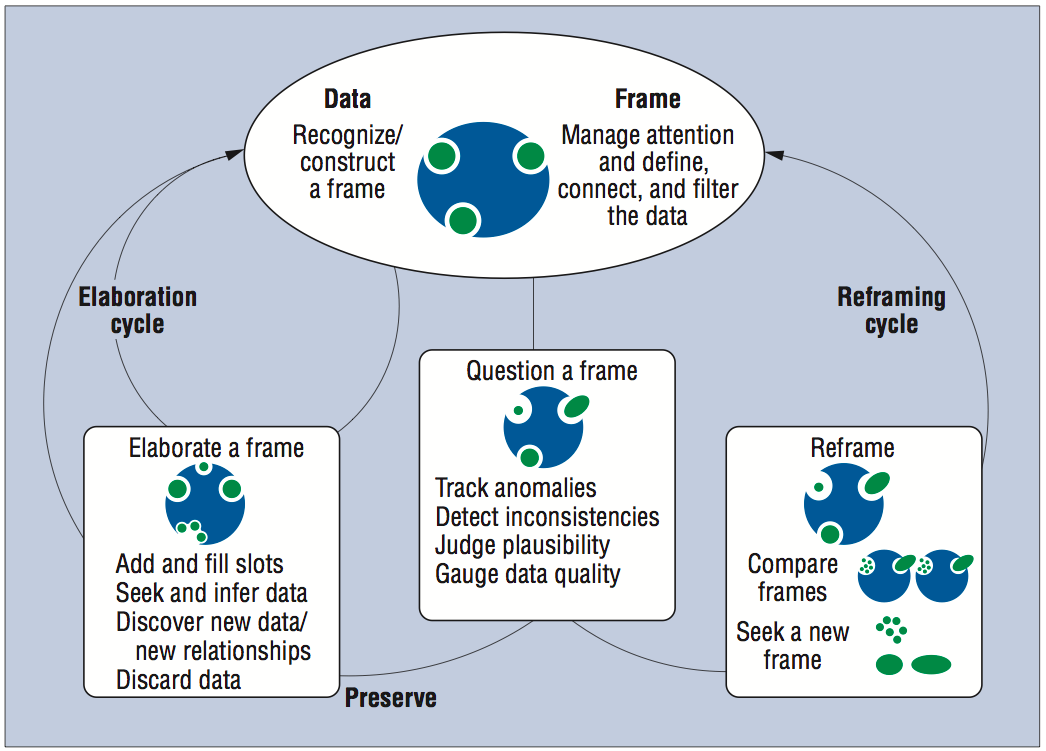
\includegraphics[width=0.75\textwidth]{images/grundlagen-data_frame_model.png}
   \caption{Data/Frame Modell nach \cite{Klein2006}}
   \label{figure:data_frame_model}
\end{figure}

% was ist dabei zu beachten?

Während des Verständnisprozesses ist es außerdem hilfreich, Wissen in irgendeiner Form externalisieren zu können, beispielsweise mit Hilfe einer Mind Map \cite{Qu2005, Novak2007, Umapathy2010}. Andere Menschen können dadurch auf bereits durchgeführte Verständnisprozesse anderer aufbauen, wobei die Struktur aber wichtiger ist als der tatsächliche Inhalt \cite{Fisher2012}.

Nachdem betrachtet wurde, wie Verständnis funktioniert, stellt sich die Frage, \emph{was} vermittelt werden soll um Menschen mit wenig InfoVis-Erfahrung zu helfen. Dazu gehört laut Grammel \cite[S. 127]{Grammel2012} unter anderem das mentale Modell des Benutzers zu verwenden, beispielsweise indem dieselben Bezeichnungen verwendet werden, und zu lehren, wie Visualisierungen verwendet und interpretiert werden.

\section{Zusammenfassung}
\label{section:grundlagen_zusammenfassung}

yay

% ###################################################
\chapter{Konzeption}
\label{chapter:konzeption}


%#####################################################
\printbibliography[title=Literaturverzeichnis]

%\printindex

\end{document}